\documentclass[UTF8,a4paper,10pt]{ctexart}
\usepackage[left=2.50cm, right=2.50cm, top=2.50cm, bottom=2.50cm]{geometry}
%页边距
\CTEXsetup[format={\Large\bfseries}]{section} %设置章标题居左

%%%%%%%%%%%%%%%%%%%%%%%
% -- text font --
% compile using Xelatex
%%%%%%%%%%%%%%%%%%%%%%%
% -- 中文字体 --
%\setmainfont{Microsoft YaHei}  % 微软雅黑
%\setmainfont{YouYuan}  % 幼圆    
%\setmainfont{NSimSun}  % 新宋体
%\setmainfont{KaiTi}    % 楷体
%\setmainfont{SimSun}   % 宋体
%\setmainfont{SimHei}   % 黑体
% -- 英文字体 --
%\usepackage{times}
%\usepackage{mathpazo}
%\usepackage{fourier}
%\usepackage{charter}

%\usepackage{helvet}

\usepackage{amsmath, amsfonts, amssymb} % math equations, symbols
\usepackage[english]{babel}
\usepackage{color}	% color content
\usepackage{graphicx}	% import figures
\usepackage{url}	% hyperlinks
\usepackage{bm} 	% bold type for equations
\usepackage{multirow}
\usepackage{booktabs}
\usepackage{epstopdf}
\usepackage{epsfig}
\usepackage{algorithm}
\usepackage{algorithmic}
\usepackage{listings}
\usepackage{xcolor}
\usepackage{booktabs}
\usepackage{zhnumber}
\usepackage{longtable}
\usepackage{subfigure}
\usepackage{float}
\usepackage{caption}
\usepackage{subfigure}
\renewcommand\thesection{\zhnum{section}}
\renewcommand \thesubsection {\arabic{section}}
\renewcommand{\algorithmicrequire}{ \textbf{Input:}}
% use Input in the format of Algorithm  
\renewcommand{\algorithmicensure}{ \textbf{Initialize:}}
% use Initialize in the format of Algorithm  
\renewcommand{\algorithmicreturn}{ \textbf{Output:}}
% use Output in the format of Algorithm  
%%%%%%%%%%%%%%%%%%
\usepackage{listings}
\usepackage{color}
\definecolor{dkgreen}{rgb}{0,0.6,0}
\definecolor{gray}{rgb}{0.5,0.5,0.5}
\definecolor{mauve}{rgb}{0.58,0,0.82}
\lstset{frame=tb,
  language=Python,
  aboveskip=3mm,
  belowskip=3mm,
  showstringspaces=false,
  columns=flexible,
  basicstyle={\small\ttfamily},
  numbers=left,%设置行号位置none不显示行号
  %numberstyle=\tiny\courier, %设置行号大小
  numberstyle=\tiny\color{gray},
  keywordstyle=\color{blue},
  commentstyle=\color{dkgreen},
  stringstyle=\color{mauve},
  breaklines=true,
  breakatwhitespace=true,
  escapeinside=``,%逃逸字符(1左面的键),用于显示中文例如在代码中`中文...`
  tabsize=4,
  extendedchars=false %解决代码跨页时,章节标题,页眉等汉字不显示的问题
}

%%%%%%%%%%%%%%%%%%%%%%%%%%%%
\usepackage{fancyhdr} %设置页眉、页脚
\pagestyle{fancy}
\lhead{}
\chead{}
%\rhead{\includegraphics[width=1.2cm]{fig/ZJU_BLUE.eps}}
\lfoot{}
\cfoot{}
\rfoot{}
\fancyfoot[RE,RO]{~\thepage~}

\fancyhead[RE,RO]{计算物理导论 \quad 2022春季学期 \quad 作业10 \quad 何翼成}

%%%%%%%%%%%%%%%%%%%%%%%
%  设置水印
%%%%%%%%%%%%%%%%%%%%%%%
%\usepackage{draftwatermark}         % 所有页加水印
%\usepackage[firstpage]{draftwatermark} % 只有第一页加水印
% \SetWatermarkText{Water-Mark}           % 设置水印内容
% \SetWatermarkText{\includegraphics{fig/ZJDX-WaterMark.eps}}         % 设置水印logo
% \SetWatermarkLightness{0.9}             % 设置水印透明度 0-1
% \SetWatermarkScale{1}                   % 设置水印大小 0-1    

\usepackage{hyperref} %bookmarks
\hypersetup{colorlinks, bookmarks, unicode} %unicode

\title{\textbf{一维朗之万方程的谐振子求解}}
\author{ 何翼成 \thanks{学号:520072910043; \newline
    邮箱地址:heyicheng@sjtu. edu. cn} }
\date{\today}

\begin{document}
\maketitle

%\begin{abstract}
%这是一篇中文小论文。这个部分用来写摘要。摘要的章标题默认是英文,还没找到改成中文的方法:(
%\end{abstract}
\section*{Project 1}
\section{题目分析}
%%%以下为插入图片模板
%\quad \newline
	\begin{figure}[!htbp]
		\centering
		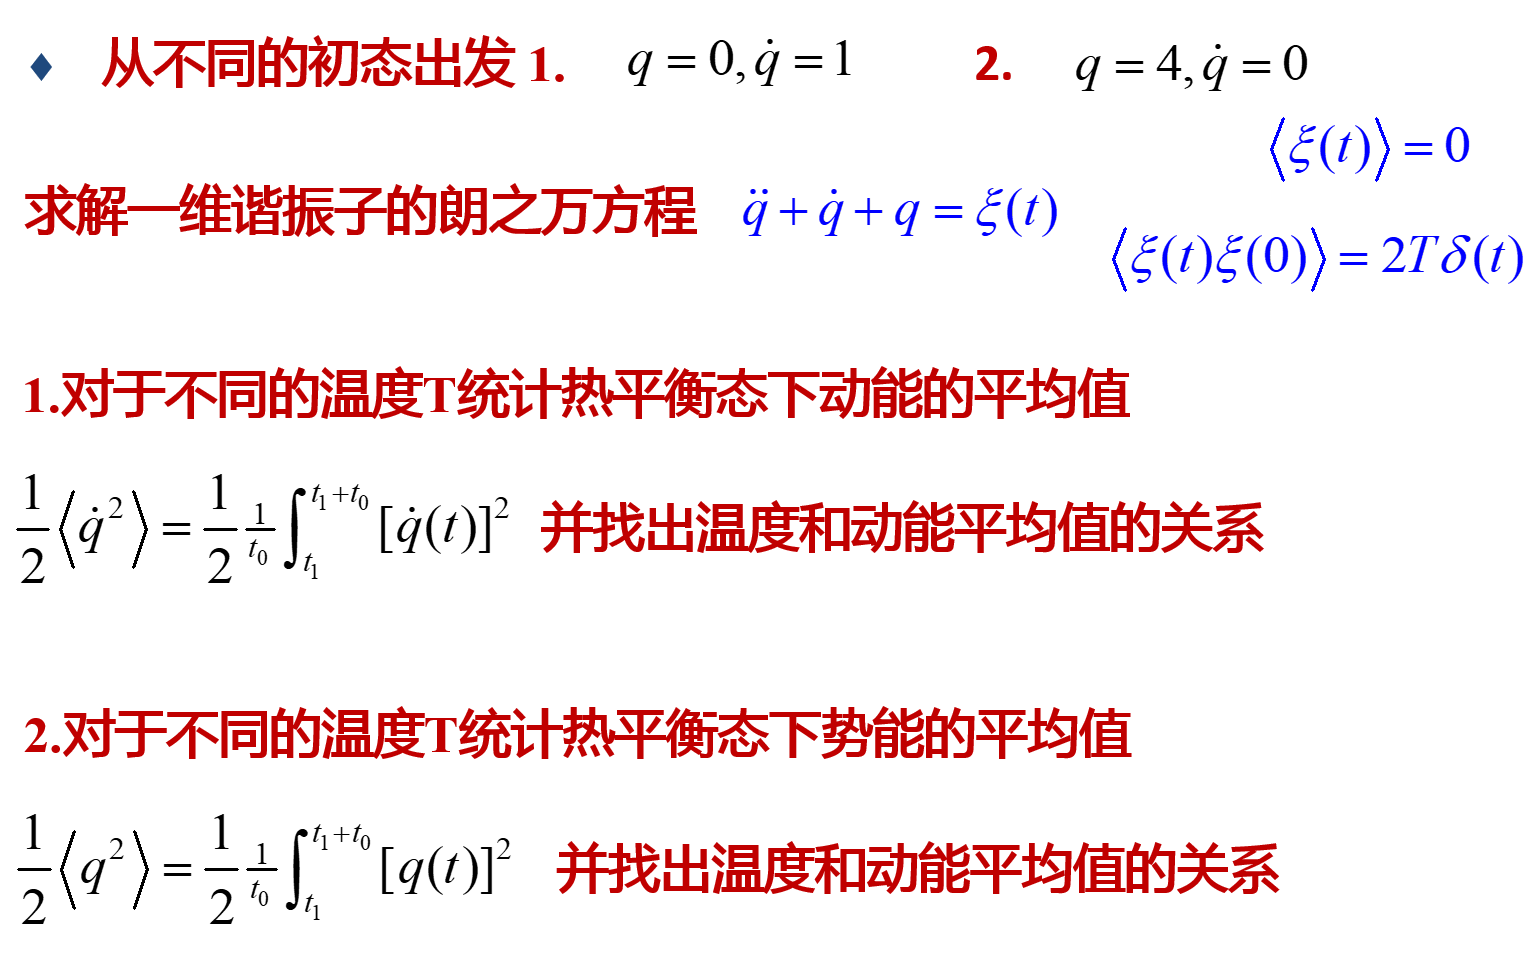
\includegraphics[width=1\textwidth,height=0.6\textwidth]{pictures/pro.png}
		\caption{题目总览} \label{project1}
	\end{figure}



\section{代码展示}
\lstset{language=matlab}
\begin{lstlisting}
    clear;clc;

    %初始条件区
    x0=0;v0=1;
    %x0=4;v0=0;
    dt=0.1;%时间间隔
    tspan=0:dt:2000;%时间序列
    T=0:0.1:300;%温度
    TXmx=zeros(length(T),length(tspan));
    TVmx=TXmx;
    avgEK=zeros(1,length(T));
    avgV=avgEK;
    m=round(1/5*length(tspan));%截取数据量
    
    %计算T-x和T-v矩阵
    for i=1:length(T)
        Ti=T(i);
        [xi,vi]=Euler(x0,v0,dt,tspan,Ti);
        TXmx(i,:)=xi;TVmx(i,:)=vi;
        %对于不同温度T的动能平均项
        avgEK(i)=avgek(vi,m);
        %对于不同温度T的势能平均值
        avgV(i)=avgv(xi,m);
        clc;
        disp("已完成第"+i+"轮计算,占比为"+i/length(T)*100+"%")
    end
    
    %绘制T-<Ek>和T-<V>图像
    figure(1)
    plot(T,avgEK,'r')
    xlabel('Temprature'),ylabel('<E_{k}>')
    figure(2)
    plot(T,avgV,'r')
    xlabel('Temprature'),ylabel('<V>')
    
    
    %函数定义区
    %步进法求x,v
    function [x,v]=Euler(x0,v0,dt,tspan,T)
        x=zeros(1,length(tspan));v=x;
        x(1)=x0;v(1)=v0;
        %计算x,t
        for i=2:length(tspan)
            x(i)=x(i-1)+v(i-1)*dt;
            v(i)=v(i-1)+(sqrt(2*T)*randn(1,1)*sqrt(dt))-(v(i-1)+x(i-1))*dt;
        end
    end
    
    %求解平均动能和势能
    function avgEk=avgek(v,m)
        id=(length(v)-m):length(v);
        avgEk=1/2*sum(v(id).^2)/m;
    end
    function avgV=avgv(x,m)
        id=(length(x)-m):length(x);
        avgV=1/2*sum(x(id).^2)/m;
    end
\end{lstlisting}

\section{结果分析与结论}
在代码中分别准备了不同的初始条件,代入不同的初始条件进行运行就可以得到对应的图像。

\subsubsection{初始条件一}
	\begin{figure}[!htbp]
		\centering
		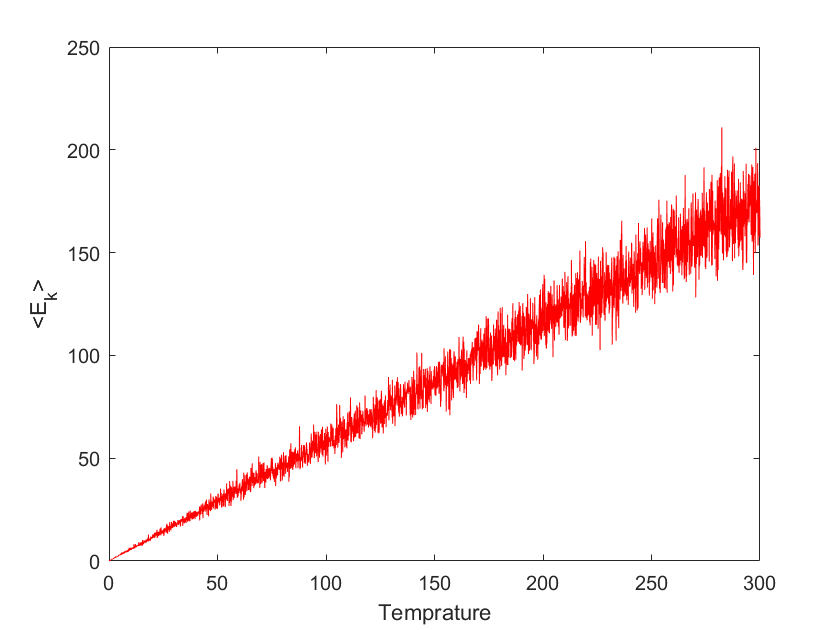
\includegraphics[width=0.4\textwidth,height=0.3\textwidth]{pictures/ek1.png}
		\caption{在初始条件一的情况下的<Ek>的演化情况>} \label{ek1}
	\end{figure}
	\begin{figure}[!htbp]
		\centering
		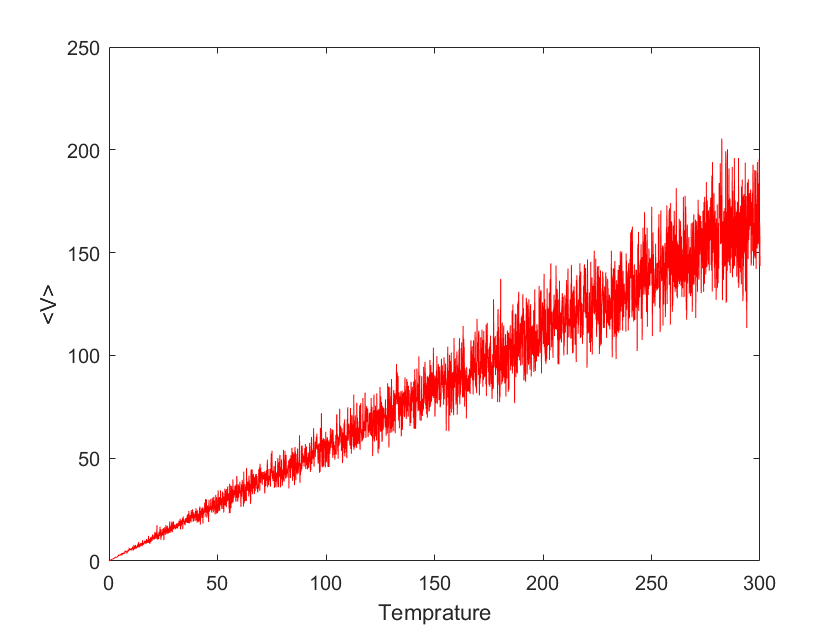
\includegraphics[width=0.4\textwidth,height=0.3\textwidth]{pictures/v1.png}
		\caption{在初始条件一的情况下的<V>的演化情况} \label{v1}
	\end{figure}
\subsubsection{初始条件二}
\begin{figure}[!htbp]
    \centering
    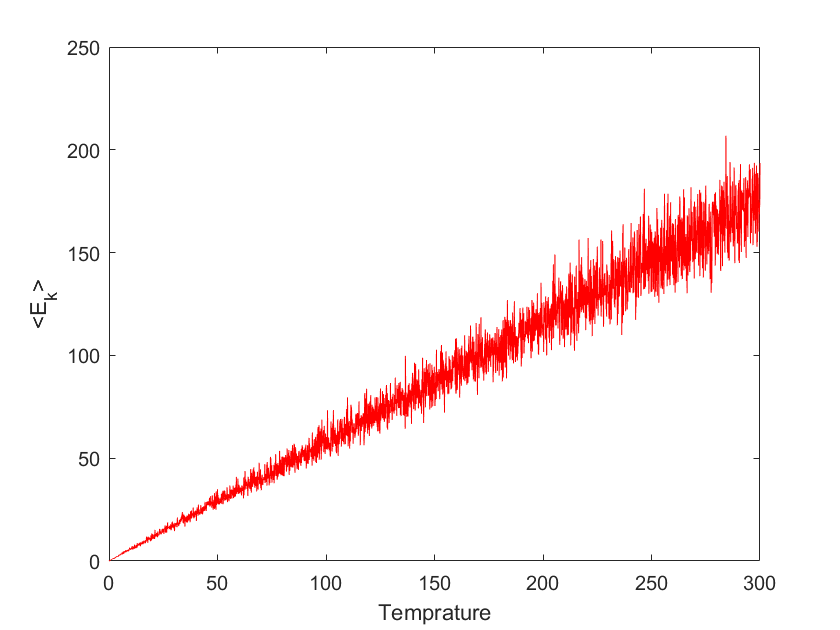
\includegraphics[width=0.4\textwidth,height=0.3\textwidth]{pictures/ek2.png}
    \caption{在初始条件二的情况下的<Ek>的演化情况>} \label{ek2}
\end{figure}
\begin{figure}[!htbp]
    \centering
    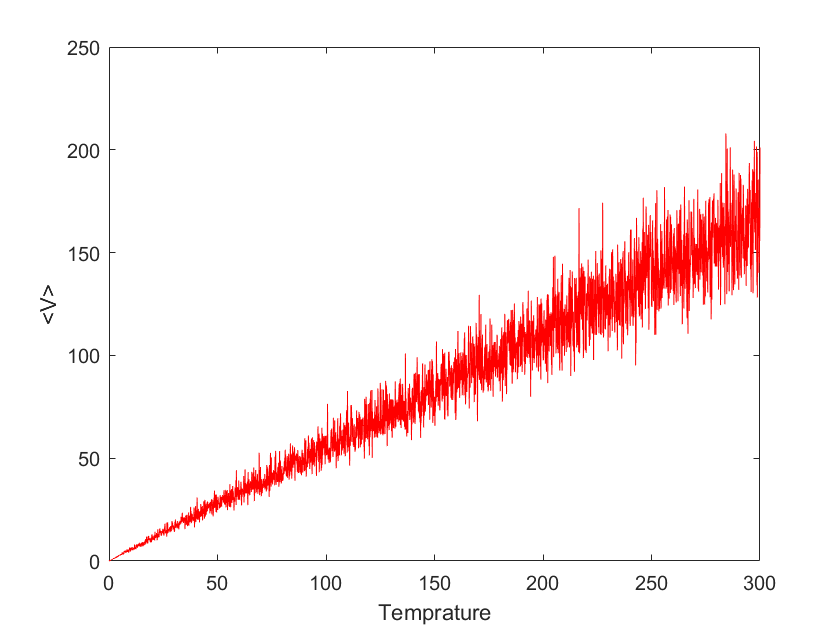
\includegraphics[width=0.4\textwidth,height=0.3\textwidth]{pictures/v2.png}
    \caption{在初始条件二的情况下的<V>的演化情况} \label{v2}
\end{figure}
\quad \newline
由上述图像可知,由于在计算时对原始方程的高度简化(各参数均取1,比如质量、玻尔兹曼常数等),所以得到的方程的解也必须要对
其结果的含义进行考量。不难发现,当玻尔兹曼常数取到1的时候,原本的能均分原理所产生的一维动能公式
$E_{k}=\frac{1}{2}k_{b}T$自然而然地化作了$E_{k}=\frac{1}{2}T$。再观察一下图像,会发现数值模拟地结果虽然沿着温度升高并不平滑,但是总体上与$y=\frac{1}{2}x$
的直线拟合非常良好。同样,对于平均势能而言,也遵循了类似的规律,其拟合同样和$y=\frac{1}{2}x$接近。

  %%%%%%%%%%%%%%%%%%%%%%%%%第二题%%%%%%%%%%%%%%%%%%%%%%%%%%%%%%%%%
  %%%%%%%%%%%%%%%%%%%%%%%%%第二题%%%%%%%%%%%%%%%%%%%%%%%%%%%%%%%%%
  %%%%%%%%%%%%%%%%%%%%%%%%%第二题%%%%%%%%%%%%%%%%%%%%%%%%%%%%%%%%%
  %%%%%%%%%%%%%%%%%%%%%%%%%第二题%%%%%%%%%%%%%%%%%%%%%%%%%%%%%%%%%
\
%以下为插入代码模板
%~\\
%\lstset{language=matlab}
%\begin{lstlisting}
%\end{lstlisting}


%%%以下为插入图片模板
%\quad \newline
%	\begin{figure}[!htbp]
%		\centering
%		\includegraphics[width=0.5\textwidth,height=0.375\textwidth]{pictures/minscale.png}
%		\caption{最小风向} \label{minsacle}
%	\end{figure}

%%%以下为插入图片模板
%\quad \newline
%	\begin{figure}[!htbp]
%		\centering
%		\includegraphics[width=0.5\textwidth,height=0.375\textwidth]{pictures/minscale.png}
%		\caption{最小风向} \label{minsacle}
%	\end{figure}

%    \begin{algorithm}
%		\caption{Title of the Algorithm}
%     	\begin{algorithmic}[1]
%			\REQUIRE some words.  % this command shows "Input"
%			\ENSURE ~\\           % this command shows "Initialized"
%			some text goes here ... \\
%			\WHILE {\emph{not converged}}
%			\STATE ... \\  % line number at left side
%			\ENDWHILE
%			\RETURN this is the lat part.  % this command shows "Output"
%		\end{algorithmic}
%	\end{algorithm}

\end{document}